\documentclass[journal]{vgtc}              


\usepackage{mathptmx}
\usepackage{graphicx}
\usepackage{times}
\usepackage{hyperref}
\usepackage{xcolor}
\usepackage{mdframed}
\usepackage{nomencl}
\makenomenclature
\usepackage{siunitx}
\usepackage{tcolorbox}
\hypersetup{
  pdfauthor = {},
  pdftitle = {},
  pdfsubject = {},
  pdfkeywords = {},
  colorlinks=true,
  linkcolor= black,
  citecolor= black,
  pageanchor=false,
  urlcolor = black,
  plainpages = false,
  linktocpage
}


\onlineid{0}
\vgtccategory{Research}
\vgtcinsertpkg



\title{Measurement Device Independent Quantum Key Distribution Network}

\author{Chris Irish and Jonathan Gough}


\abstract
{
With the every advancing development of quantum computation and its ability to breech current security protocols, new approaches to quantum cryptography must be developed. One such approach is \textit{Measurement Device Independent Quantum Key Distribution}. Up until now, MDIQKD has been largely theoretical. For the first MDIQKD has been experimentally verified by researchers from China. A three user, four node MDIQKD network was achieved within the city of Hefei. A \textcolor{orange}{\textbf{"step in the right direction towards a secure global network"}} says one leading MDIQKD theorist.
}

\keywords{MDIQKD, QKD, BB84}


\CCScatlist{
}

  \teaser{ 
 \centering
 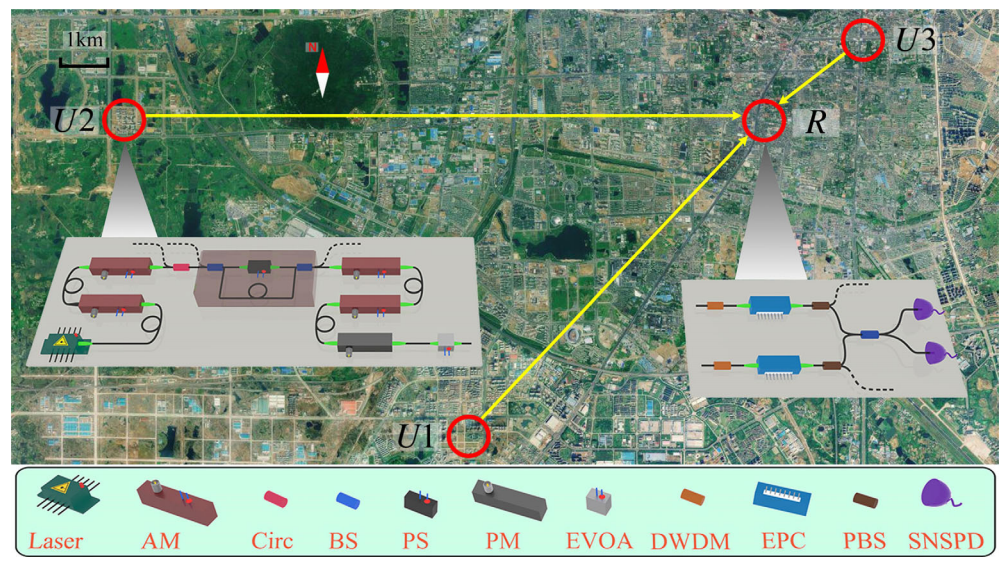
\includegraphics[width=16cm]{map}
  \caption{Birds-eye view of the MDIQKD network topology\cite{PhysRevX.6.011024}.}
  }



\begin{document}


\firstsection{QKD great}

\maketitle

Alt: One area in which… is cyber security, where the
muscular prime factorisation prowess is predicted to make
a merry mockery of our best existing secret-key methods. /
The emergence of Quantum Computing has thrown the
world of cyber-security up in the air.
While the muscular/barbaric prime factorisation abilities of
quantum computers seem set to make a mockery of our
best existing cyber-security measures, study of quantum
communications has unearthed a prospective lifeline in the
form of a brand new, watertight security key method,
whose integrity against eavesdroppers is guaranteed in
cast iron by the laws of quantum physics.
----
Meet Eve, the cardboard eavesdropper. She lurks in every
theoretical communication model, able to instantly
recognise any potential weakness, and call on any
technological trinket to exploit it. A sleek and savage
predator on a single-minded hunt for illicit data. Intent on
maximum personal damage to our two communicators,
Alice and Bob, be it financially, physically, or emotionally.
Every
----
In reality we also need to contend with interference from
the environment - everything else in the world that
interacts with our qubit (be it coded to the spin of an ion, or
photon, or to any quantum-behaved property we can
decompose in a suitable binary way.
Of course, everything else might also include malicious
tampering by Eve, the customary cardboard
eavesdropper, intent on nothing other that maximum
personal damage to Alice and Bob, the rando schlubs
sharing a secret code, physically, socially, emotionally,
using any and all the data she can leech from the cracks
in their quantum network



\section{but QKD issues}
\textcolor{orange}{\textbf{"There is no thing as security if it always requires some assumptions"}}. Dr Lluis Masanes,  A leading researcher on quantum information sciences at UCL has his doubts on standard QKD network security.   

\vspace{0.3cm}

\noindent Previous demonstrations of a \textit{quantum key distribution} (QKD) networks, such as by the team at moscow state university\cite{2017QuEle..47..798K} , have been achieved but are vulnerable to an attack by Eve. Standard QKD networks (also known as prepare and measure QKD networks) have to assume the central relays to be completely trustful. In reality this is extremely unlikely due various security loopholes associated with these networks. One such security loophole is the \textit{detection loophole}. The \textit{detection loophole} is caused by unavoidable losses in the quantum channel and  the coupling between photon source and optical fibres. Additionally losses occur due to the measurement devices finite detection efficiency. This flaw can allow Eve to perform an \textit{intercept and resend} attack, in which Eve intercepts and measures the state being transmitted and prepares a fake state to be sent to Bob.

\section{MDIQKD resolve issues associated with QKD}


A MDIQKD network attempts to close the \textit{detection loophole} by \textcolor{red}{removing the measurement devices entirely} and instead uses a shared  central station to create entanglement-like correlations between Alice and Bob through a \textit{Bell-state measurements}(BSM). This approach is based of \textit{time-reversed entanglement based QKD}\cite{PhysRevA.54.2651}. The bell state measurement provides a vital piece of information that when combined with the outgoing information, it allows the network users to work out what information is being sent to them. As only the network user knows his/her outgoing information, even if Eve completely controls the central station she can not gain any information about the cryptographic key. For a MDIQKD network to be successful it requires that the network users have almost perfect state preparation (fully know what their outgoing information is). However this issue is easily addressed as their states can be experimentally verified in a fully protected laboratory environment, outside of Eve's interference.  

QKD networks can be characterised by their \textit{secure key rate}.  The secure key rate gives a measure of how much secure information (measured in bits) is transmitted per second by the network. It is calculated from the networks gain rates, error rates and error correction efficiency. The secure key rate is distinct from the \textit{key rate} which only gives a measure of how much information is transmitted per second by the network. Compared to standard QKD networks the key rate for an MDIQKD network is relativity low. Under the same experimental parameters a decoy \textit{BB84 system} with a trustful relay can generate a key rate around 1000bps \textcolor{red}{over 25 times greater than the team achieved in the MDIQKD network}. However, what a MDIQKD network lacks in key rate it makes up with security. Hence, the secure key rate achieved by the team are at least 10 times higher than previous state of the art field tests.

\vspace{0.3cm}

\noindent Prof Alessio Serafini, professor of theoretical physics at UCL reinforced the importance of the teams work for the theory of quantum information.

\vspace{0.3cm}

\textcolor{orange}{\textbf{" The theory becomes true when you build a machine with it and Device Independence is very instrumental to this because it tells you this machines can only be quantum, that's in the end what it is.".}}

\section{But MDIQKD also has issues}

Upgrading a standard QKD network to a MDIQKD network has not been attempted until now as there are two main technical challenges that arise. The first being \textit{reference frame calibration}. This refers the the real time alignment of reference frames between network users. In past attempts to achieve \textit{reference frame calibration} researcher have used additional fibre links between users. The results of this is that the demand of fibre links increases quadratically with the number of network users. This is impractical when scaling up to a city sized user populations. A solution was found by the researchers in China through a \textit{phase feedback scheme}. This allowed for a far more manageable linear scaling of fibre links with the number of network users.

The second technical challenge involves \textit{maintaining indistinguishability} between the network users. In a MDIQKD network any two users can be switched upon request. The new user's signals must be calibrated immediately to disallow the new and old users signals from mixing. Mixing two users signals would result in the timing, spectrum and polarization mode being indistinguishable between the two users. A solution was developed using \textit{multi-user HOM interference} technology. The team believes this technology can find applications in \textit{multi-party entanglement swapping-based quantum communication} and a \textit{quantum computing cloud}.


\begin{tcolorbox}
\section{Box 1: Typical MDIQKD Process}

1. Alice and Bob both prepare outgoing signals in the four possible polarization states.\\
2. Alice and Bob both send their states to the central relay via optical fibres.\\
3. The central relay performs a bell state measurement that projects the incoming signals into a bell state.\\
4. The relay publicly announces the bell state.\\
5. Alice and Bob then publicly announce there basis but not there associated bits.\\
6. From the relays bell state, Alice/Bobs basis and knowing there own outgoing bit. Alice/Bob can work out the opposite parties bit that was sent.\\
7. Process is repeated until cryptographic keys are built up.

\end{tcolorbox}

\begin{tcolorbox}
\section{Box 2: So what QKD?}

In the same way that we can decompose a 2D graph into
x and y coordinated, so too can we decompose any spin
representation into x, y, and z components. (fig). each of
which can be either in the up or down state when
measured.
A state that is prepared to be ‘up’ in one direction, z, for
instance, would be measured as ‘up’ with 100% probability
if we align our measurement device to the z-direction, but
would be measured as ‘up’ or ‘down’ with equal
probability, if we measure in either the ‘x’ or ‘y’ directions.
With any orientation we choose, we can name a
z-direction, for instance, and prepare an ion, electron, or
photon with spin is (prepared to be) aligned perfectly up
or down in an arbitrary x-direction, will be poised exactly in
between up and down if measured in the y- or x-directions.

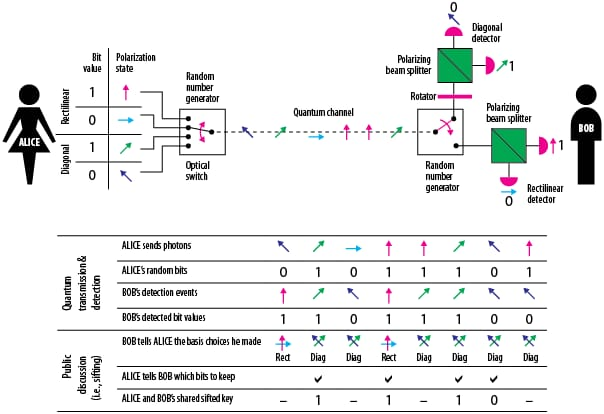
\includegraphics[width=\linewidth]{Box_2}

\end{tcolorbox}


\section{Experts opinions and next steps}


Dr Lluis Masanes also has some doubts on the security of physical MDIQKD networks (shown below). 

\vspace{0.3cm}

\textcolor{orange}{\textbf{"In the defence of the device independent, it is easy to say  that it Is the most secure framework. But in a given that you define the problem in a way that it is possible at all to do it. Okay, if my device broadcast my secret key. Yeah. I mean, it doesn't matter what you do, it's impossible (to achieve absolute security )".}}

\vspace{0.3cm}

\noindent Instead some research groups are proposing \textit{Semi Device Independence} in an attempt to balance theoretical ambitions and practical constraints. Here the network users only trust certain devices known to be secure. 

  






\bibliographystyle{unsrt}  
\bibliography{references}

\end{document}
